Para esta sección del trabajo practico el objetivo es determinar la frecuencia de resonancia $w_0$ del circuito planteado en la figura~\ref{fig:exp3}. Y a partir de esto determinar el valor de la inductancia.

\begin{figure}[H]
    \centering
    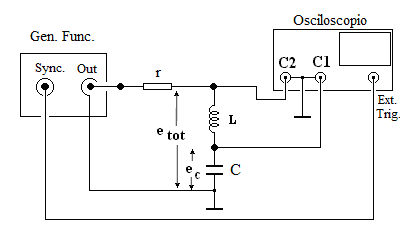
\includegraphics[width=0.7\linewidth]{Imagenes/exp3.png}
    \caption{Circuito experimento 3}
    \label{fig:exp3}
\end{figure}

Para modelizar detalladamente el comportamiento del circuito y además, para determinar el valor de la resistencia $r$ se debe tener en cuenta el efecto que este tiene sobre la frecuencia de resonancia, por consiguiente se debe plantear el análisis de la siguiente manera:
\begin{equation}
        I_{\mathscr{s}}=\frac{V_{\scr{s}}}{\scr{Z}_{t\scr{s}}}
        \begin{cases}
            \scr{H}_{1\scr{s}}=\frac{1}{\scr{Z}_{t\scr{s}}}\cdot [\scr{s}L+\frac{1}{\scr{s}C}]\\

            \scr{H}_{2\scr{s}}=\frac{1}{\scr{Z}_{t\scr{s}}}\cdot \frac{1}{\scr{s}C}
        \end{cases}
\end{equation}
La impedancia total del circuito $\scr{Z}_{t\scr{s}}$ es por ende:
\begin{equation}
\begin{aligned}
     \scr{Z}_{t\scr{s}}=\scr{s}L+r+\frac{1}{\scr{s}C}\lrah \scr{Z}_{t\scr{s}}^{-1}&=\frac{1}{\scr{s}L+r+\frac{1}{\scr{s}C}}\\
     &=\frac{1}{L}\cdot\frac{\scr{s}}{\scr{s}^2+\scr{s}\frac{r}{L}+\frac{1}{LC}}
\end{aligned}
\end{equation}
Teniendo la impedancia general del circuito se pudo obtener las siguientes expresiones:
\begin{equation}\label{eq:ftexp3}
    \begin{cases}
        \scr{H}_{1\scr{s}}=\frac{\scr{s}^2+\frac{1}{LC}}{(\scr{s}^2+\frac{r}{L}\scr{s}+\frac{1}{LC})}\cdot \\
        \\
        \scr{H}_{2\scr{s}}=\frac{1}{\scr{s}^2+\frac{r}{L}\scr{s}+\frac{1}{LC}}\cdot \frac{1}{LC}
    \end{cases}
\end{equation}

A partir de estas funciones de transferencia es de esperar que los diagramas de Bode de este circuito sean similar a lo trazado a continuación:
\begin{figure}[H]
    \begin{minipage}{0.49\textwidth}
       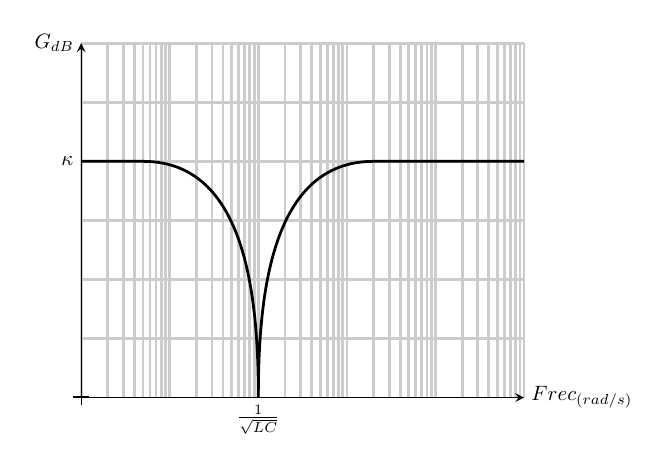
\begin{tikzpicture}[scale=0.75,every node/.style={transform shape}]

    \def\scalya{0}%Desfase curvas
    \def\scaly{1/5}%Escala eje y
    \def\scalx{1.5}%Escala eje x
    \def\scalxa{3}%Desfase puntos kHz
    
   
    
    %Ejex
    \foreach \x [evaluate={\a=int(\x+1)}]in {0,...,4}{
    \foreach \y in {1,...,10}
        \draw[line width=1pt,gray!40] ({(\x+log10(\y))*\scalx},0)--({(\x+log10(\y))*\scalx},6);
    }
    \draw[|-stealth] (0,0)--(5*\scalx,0) node[right] {$Frec_{(rad/s)}$};
    
    %Ejey
    \foreach \y [evaluate={\a=int(\y/(\scaly))}] in {1,...,6}{
        \draw[line width=1pt,gray!40] (0,\y)--(5*\scalx,\y);
    }
   \draw[|-stealth] (0,0)--(0,6) node[left]{$G_{dB}$};
   \draw[line width=1pt,black](0,4)node[left]{$\kappa$}--(0.7*\scalx,4)to[out=0,in=90](2*\scalx,0)to[out=90,in=180](3.3*\scalx,4)--(5*\scalx,4) (3,0)node[below]{$\frac{1}{\sqrt{LC}}$};
\end{tikzpicture}

\caption*{$\scr{H}_{1\scr{s}}$}
   \end{minipage}
   \begin{minipage}{0.49\textwidth}
       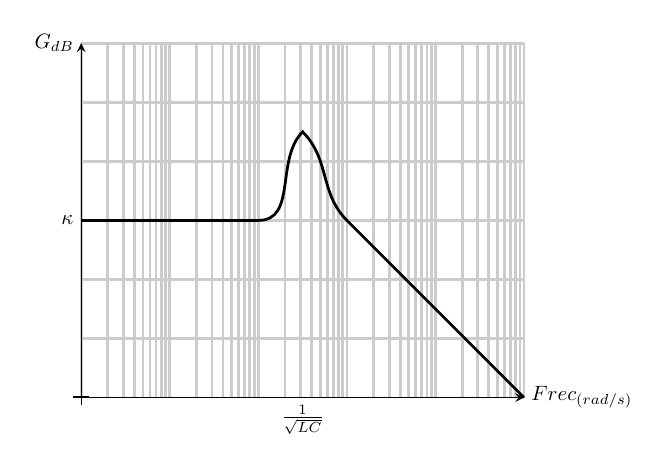
\begin{tikzpicture}[scale=0.75,every node/.style={transform shape}]

    \def\scalya{0}%Desfase curvas
    \def\scaly{1/5}%Escala eje y
    \def\scalx{1.5}%Escala eje x
    \def\scalxa{3}%Desfase puntos kHz
    
   
    
    %Ejex
    \foreach \x [evaluate={\a=int(\x+1)}]in {0,...,4}{
    \foreach \y in {1,...,10}
        \draw[line width=1pt,gray!40] ({(\x+log10(\y))*\scalx},0)--({(\x+log10(\y))*\scalx},6);
    }
    \draw[|-stealth] (0,0)--(5*\scalx,0) node[right] {$Frec_{(rad/s)}$};
    
    %Ejey
    \foreach \y [evaluate={\a=int(\y/(\scaly))}] in {1,...,6}{
        \draw[line width=1pt,gray!40] (0,\y)--(5*\scalx,\y);
    }
   \draw[|-stealth] (0,0)--(0,6) node[left]{$G_{dB}$};
   \draw[line width=1pt,black](0,3)node[left]{$\kappa$}--(2*\scalx,3)to[out=0,in=225](2.5*\scalx,4.5)to[out=-45,in=135](3*\scalx,3)--(5*\scalx,0) (2.5*\scalx,0)node[below]{$\frac{1}{\sqrt{LC}}$};
  

\end{tikzpicture}
\caption*{$\scr{H}_{2\scr{s}}$}
   \end{minipage}
   \caption{Diagramas de Bode para de las funciones de transferencia $\scr{H}_{1\scr{s}}$ y $\scr{H}_{2\scr{s}}$}
   \label{fig:BodeTransExp3}
\end{figure}


 Obtenido las funciones de transferencia se puede determinar que la frecuencia de resonancia y el factor de atenuación de nuestro circuito se pude determinar analizando la expresión $\scr{s}^2+\frac{r}{L}\scr{s}+\frac{1}{LC}$ (la parte de la función de transferencia que modeliza un comportamiento oscilatorio). Las raíces de este polinomio darán como resultado los polos de la función, teniendo en cuenta la resolución para un polinomio cuadrado perfecto, se pudo deducir que el segundo termino debe ser igual a el doble de la frecuencia $w_0$ multiplicado por un factor de corrección $\scr{E}$:
\begin{equation}
2\scr{E}w_0=\frac{R}{L} \lrah \scr{E}=\frac{r}{2}\sqrt{\frac{C}{L}}
\end{equation}

Obteniendo los polos de esta función se dedujo lo siguiente:
 \begin{equation}
     \scr{s}^2+\frac{r}{L}\scr{s}+\frac{1}{LC}
     \begin{cases}
         \scr{w}_0=\frac{1}{\sqrt{LC}}\\
         \\
         \alpha\pm jw_{c}=2w_0(-\scr{E}+j\sqrt{1-\scr{E}^2})
     \end{cases}
 \end{equation}

El efecto de sobre-tensión esta directamente asociado a la parte imaginaria y inversamente relacionada con la parte real de la expresión anteriormente expuesta. El factor de corrección varia entre $0\leq\scr{E}<1$, ya que si $\scr{E}$ es igual o superior a 1 la parte imaginaria del polo cesa de existir y el polo pasa a ser doble sobre el eje real (el efecto de atenuación excede el intercambio de energía entre los elementos).

Por lo tanto reduciendo el coeficiente $\scr{E}$ obtendremos un efecto mayor de sobre-tensión facilitando las mediciones. Teniendo en cuenta que el único elemento del circuito intercambiable es la resistencia $r$ se obtuvo la siguiente expresión:
\begin{equation}
    r=2\scr{E}\cdot\sqrt{\frac{L}{C}}
\end{equation}

Fijando el factor de corrección a un valor conveniente de $\scr{E}=0.1$ se calculo que el valor de la resistencia debía de ser de $r\approx 100~\Omega$.

Además a partir de las funciones de transferencias planteadas en la ecuación \ref{eq:ftexp3} se puede deducir que:
\begin{equation}
    f_{res} = \cfrac{1}{2 \pi \cdot \sqrt{L \cdot C}}
  \hspace{5mm}\Longrightarrow\hspace{5mm}
    L = \cfrac{1}{{\left( 2\pi \cdot f_{res} \right)}^2 \cdot C} 
\end{equation}

\unsubsubsection{Mediciones}
Para este experimento se utilizo una de las múltiples placas suministrados por el pañol del laboratorio del departamento de electrónica.
\begin{figure}[H]
    \centering
    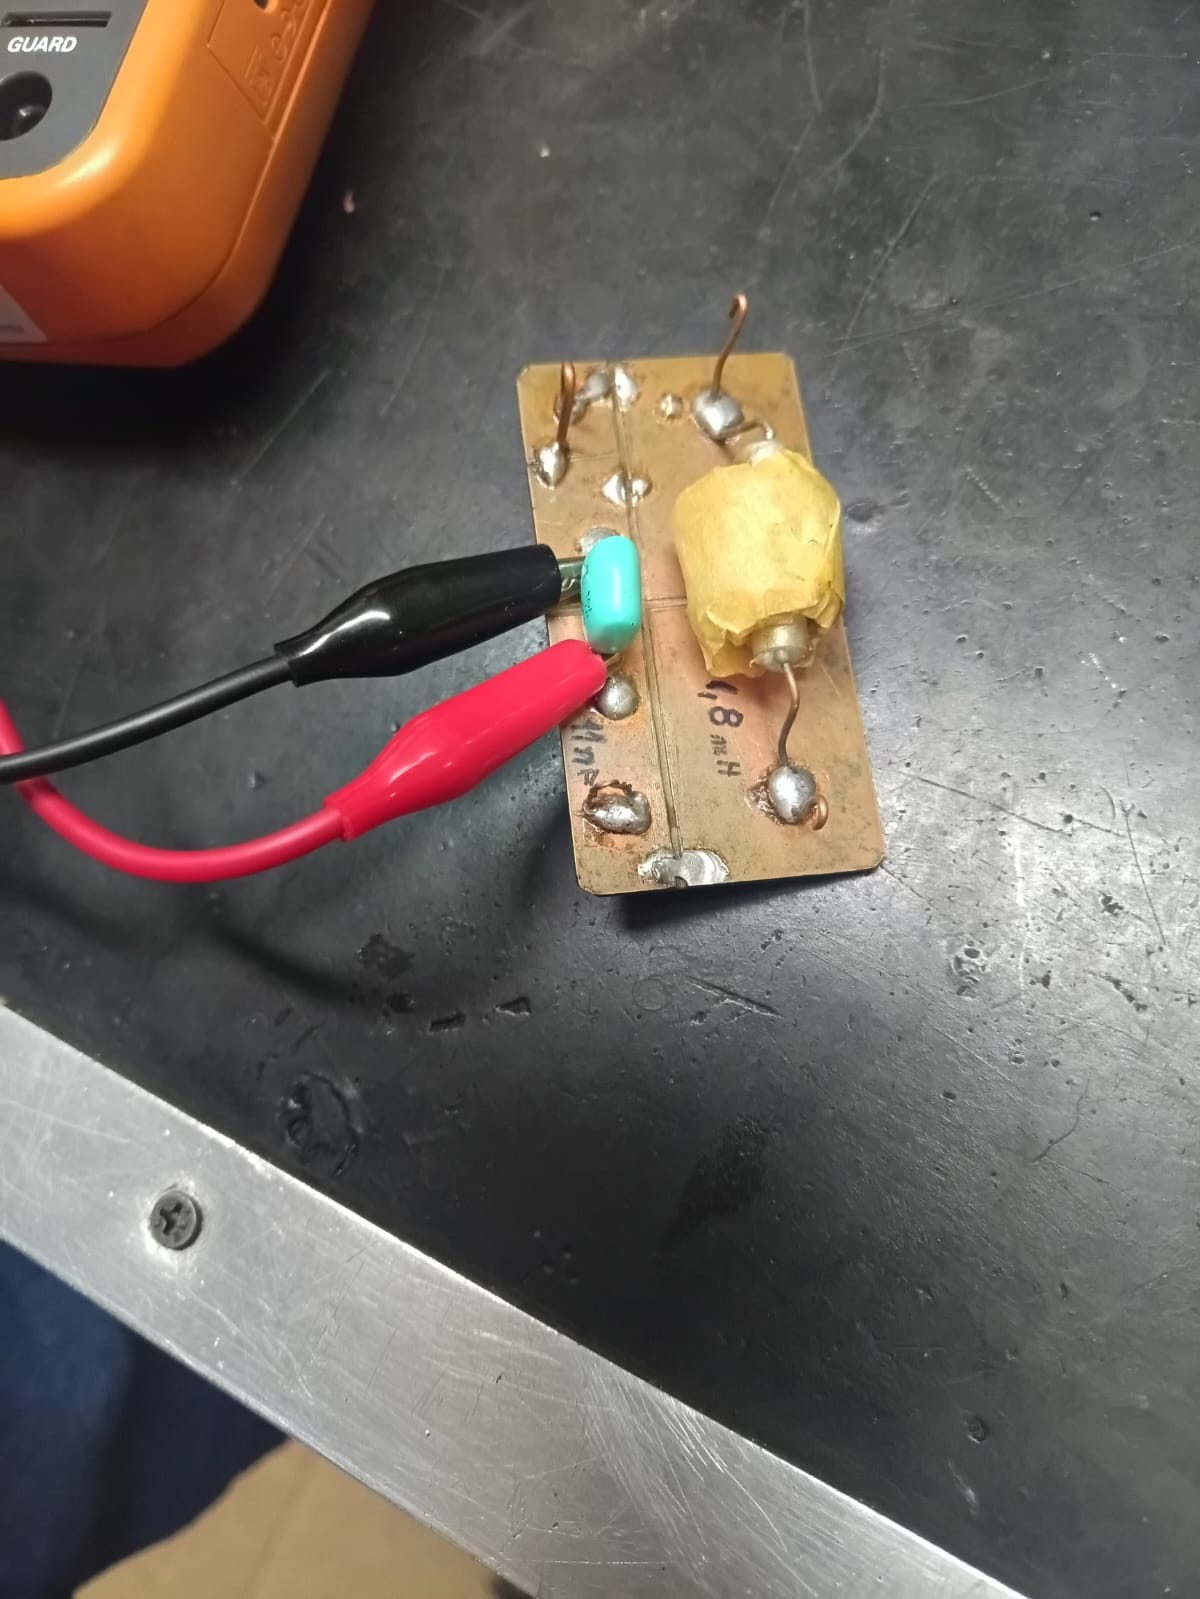
\includegraphics[width=0.6\textwidth,trim={1cm 20cm 4cm 10cm},clip]{Imagenes/CircExp3.jpeg}
    \caption{Circuito del experimento 3}
\end{figure}
\begin{equation*}
    C_{nom} = 11 ~nF  
    \hspace{2cm}
    L_{nom} = 1.8 ~mH
    \hspace{2cm}
    F_{0~calc}=35.77~KHz
\end{equation*}

Como se puede apreciar en la figura~\ref{fig:BodeTransExp3}, existe un efecto de sobre-tensión apreciable si se mide sobre el capacitor.
Tomando los valores de los componentes, los diagramas de Bode simulados son los siguientes:

\begin{figure}[H]
    \centering
    \begin{minipage}{0.49\textwidth}
        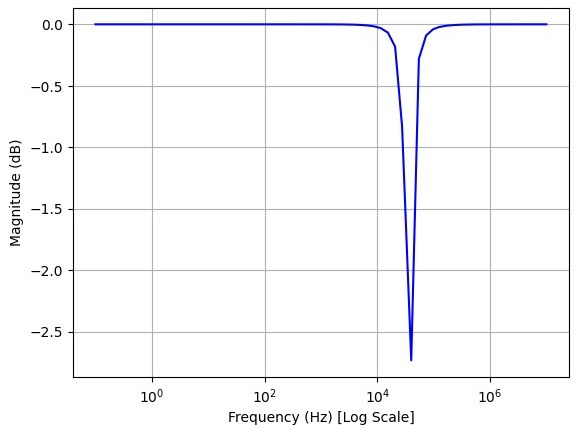
\includegraphics[width=\textwidth]{Imagenes/BodeExp3H1Mod.jpeg}
        \caption*{Modulo}
    \end{minipage}
    \begin{minipage}{0.49\textwidth}
        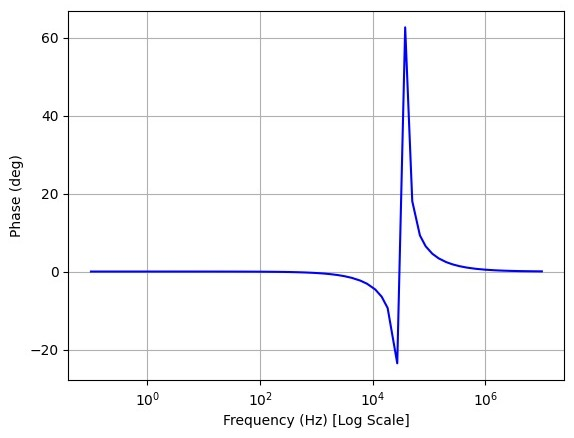
\includegraphics[width=\textwidth]{Imagenes/BodeExp3H1Arg.jpeg}
        \caption*{Fase}
    \end{minipage}
    \caption{Simulación de la función de transferencia $\scr{H}_{1\scr{s}}$}
\end{figure}
\begin{figure}[H]
    \centering
    \begin{minipage}{0.49\textwidth}
        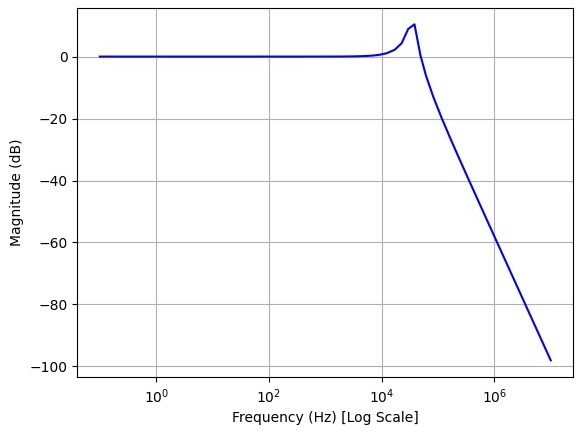
\includegraphics[width=\textwidth]{Imagenes/BodeExp3H2Mod.jpeg}
        \caption*{Modulo}
    \end{minipage}
    \begin{minipage}{0.49\textwidth}
        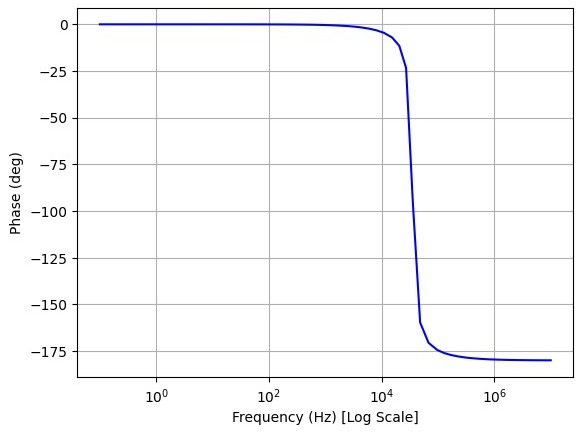
\includegraphics[width=\textwidth]{Imagenes/BodeExp3H2Arg.jpeg}
        \caption*{Fase}
    \end{minipage}
    \caption{Simulación de la función de transferencia $\scr{H}_{2\scr{s}}$}
\end{figure}
Las mediciones correspondientes a este experimento son las siguientes:
\begin{figure}[H]
    \centering
    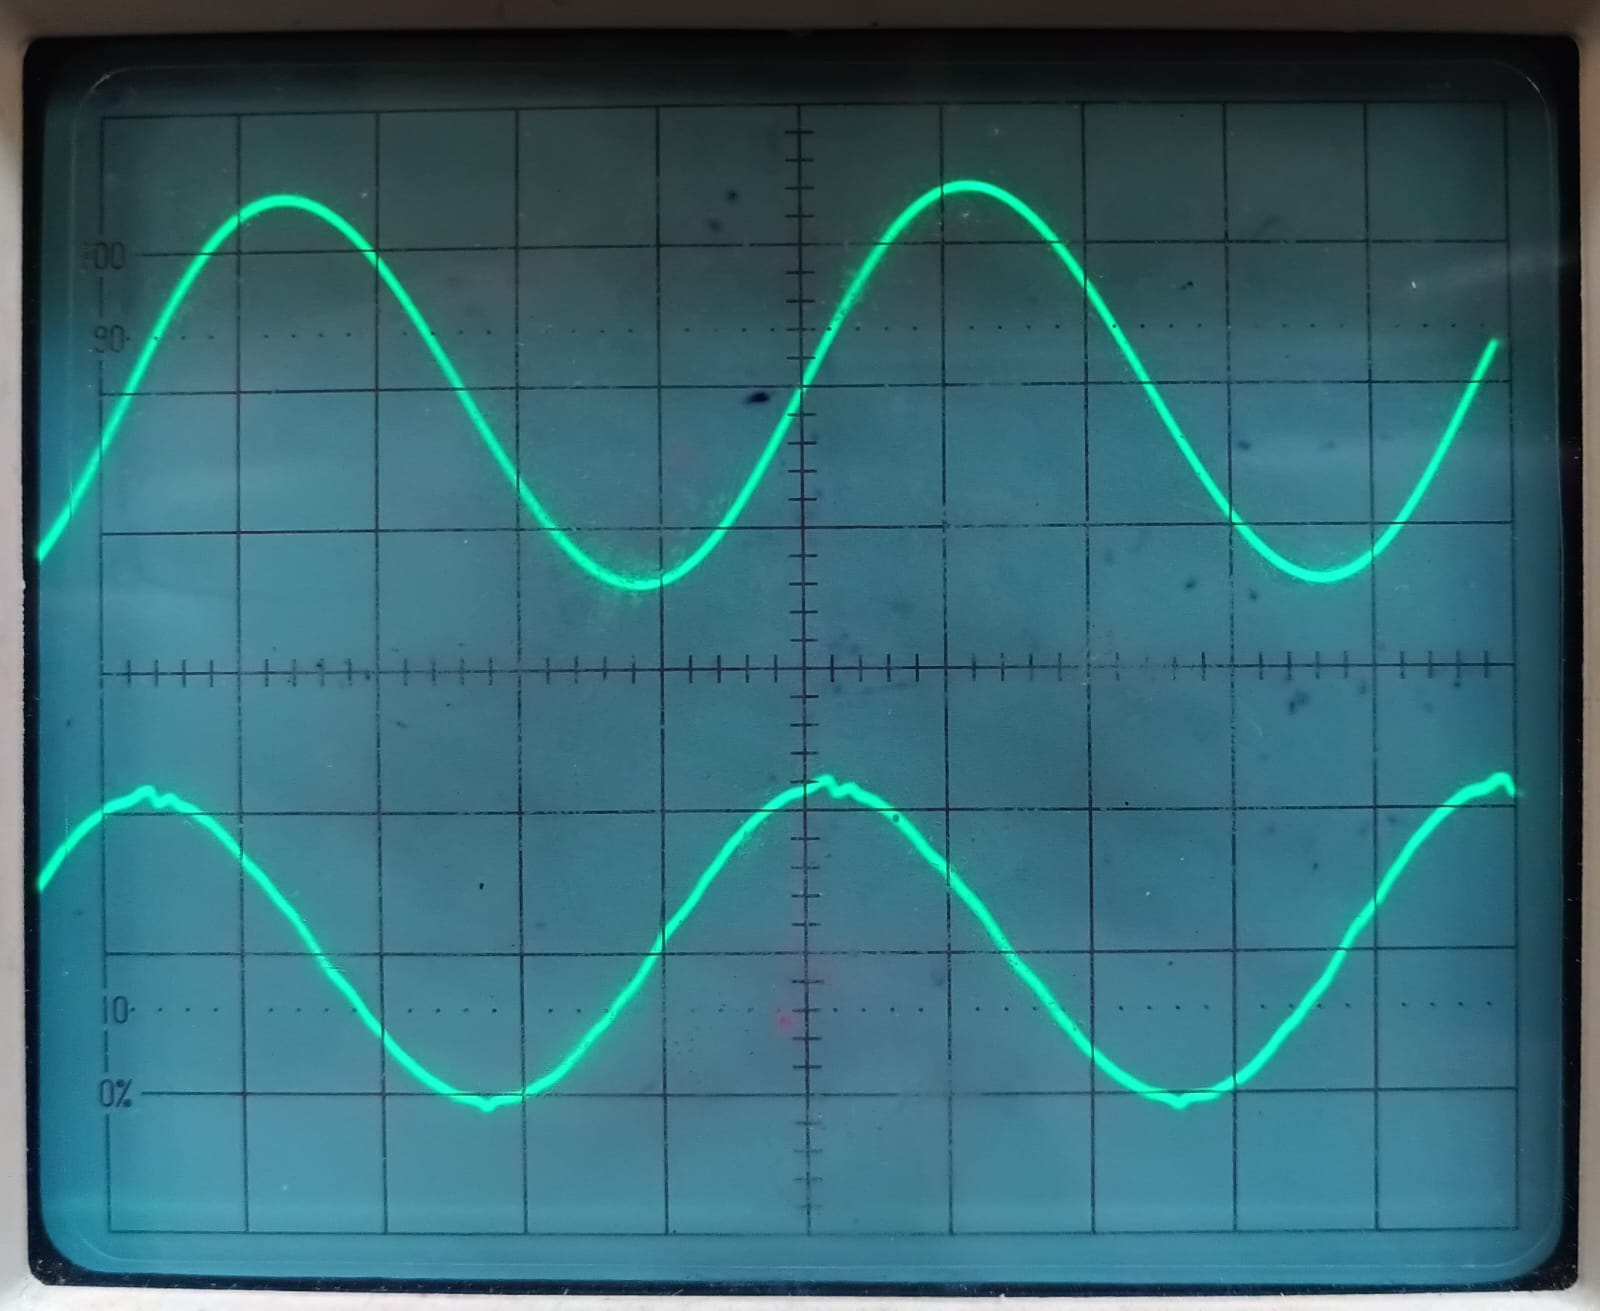
\includegraphics[width=0.6\textwidth]{Imagenes/MedExp3.jpeg}
    \caption{Señal en C1 (sup.) vs. en C2 (inf.), para frecuencia de resonancia}
\end{figure}

%Aquí se aprecia que hay un desfase de 90° entre la señal de tensión en sobre toda la rama LC y la medida sobre el capacitor, cuando la frecuencia de la señal es igual a la frecuencia de resonancia del circuito. Este atraso de 90°, es debido al inductor 

\begin{table}[H]
    \centering
    \begin{tabular}{|c|c|c|c|c|}
    \hline
        Condición & $f~[kHz]$ & $e_c$~[$V_{pp}$] & $e_{total}$~[$V_{pp}$] & $Q = \cfrac{e_c}{e_{tot}}$ \\
    \hline
        $f_2(0.707 \cdot e_{c_{max}})$ & 40.8 & 28.28 & 11.6 & - \\ 
    \hline
        $f_0(e_{c_{max}})$ & 32.6 & 39 & 9.6 & 4.06 \\ 
    \hline
        $f_1(0.707 \cdot e_{c_{max}})$ & 20.8 & 28.28 & 19 & - \\ 
    \hline    
    
        \end{tabular}
        \def\tablename{Tabla} 
        \caption{Tabla del efecto de sobre-tensión}
        \label{tab:exp3}
\end{table}


\begin{equation*}
    B = f_2 - f_1 = 20~KHz
    \hspace{2cm}
    \cfrac{f_0}{Q} = %\begin{cases}
        %16.74~KHz\\
        8.02~KHz
        %\\
        %13.978~KHz\\
    %\end{cases}
    \hspace{2cm}
    L_{calc}=2.167~mH
\end{equation*}

\unsubsubsection{Comprobación}
Se utilizo un medidor LRC para comprobar los valores de los componentes: 
\begin{figure}[H]
    \begin{minipage}{0.49\textwidth}
    \centering
    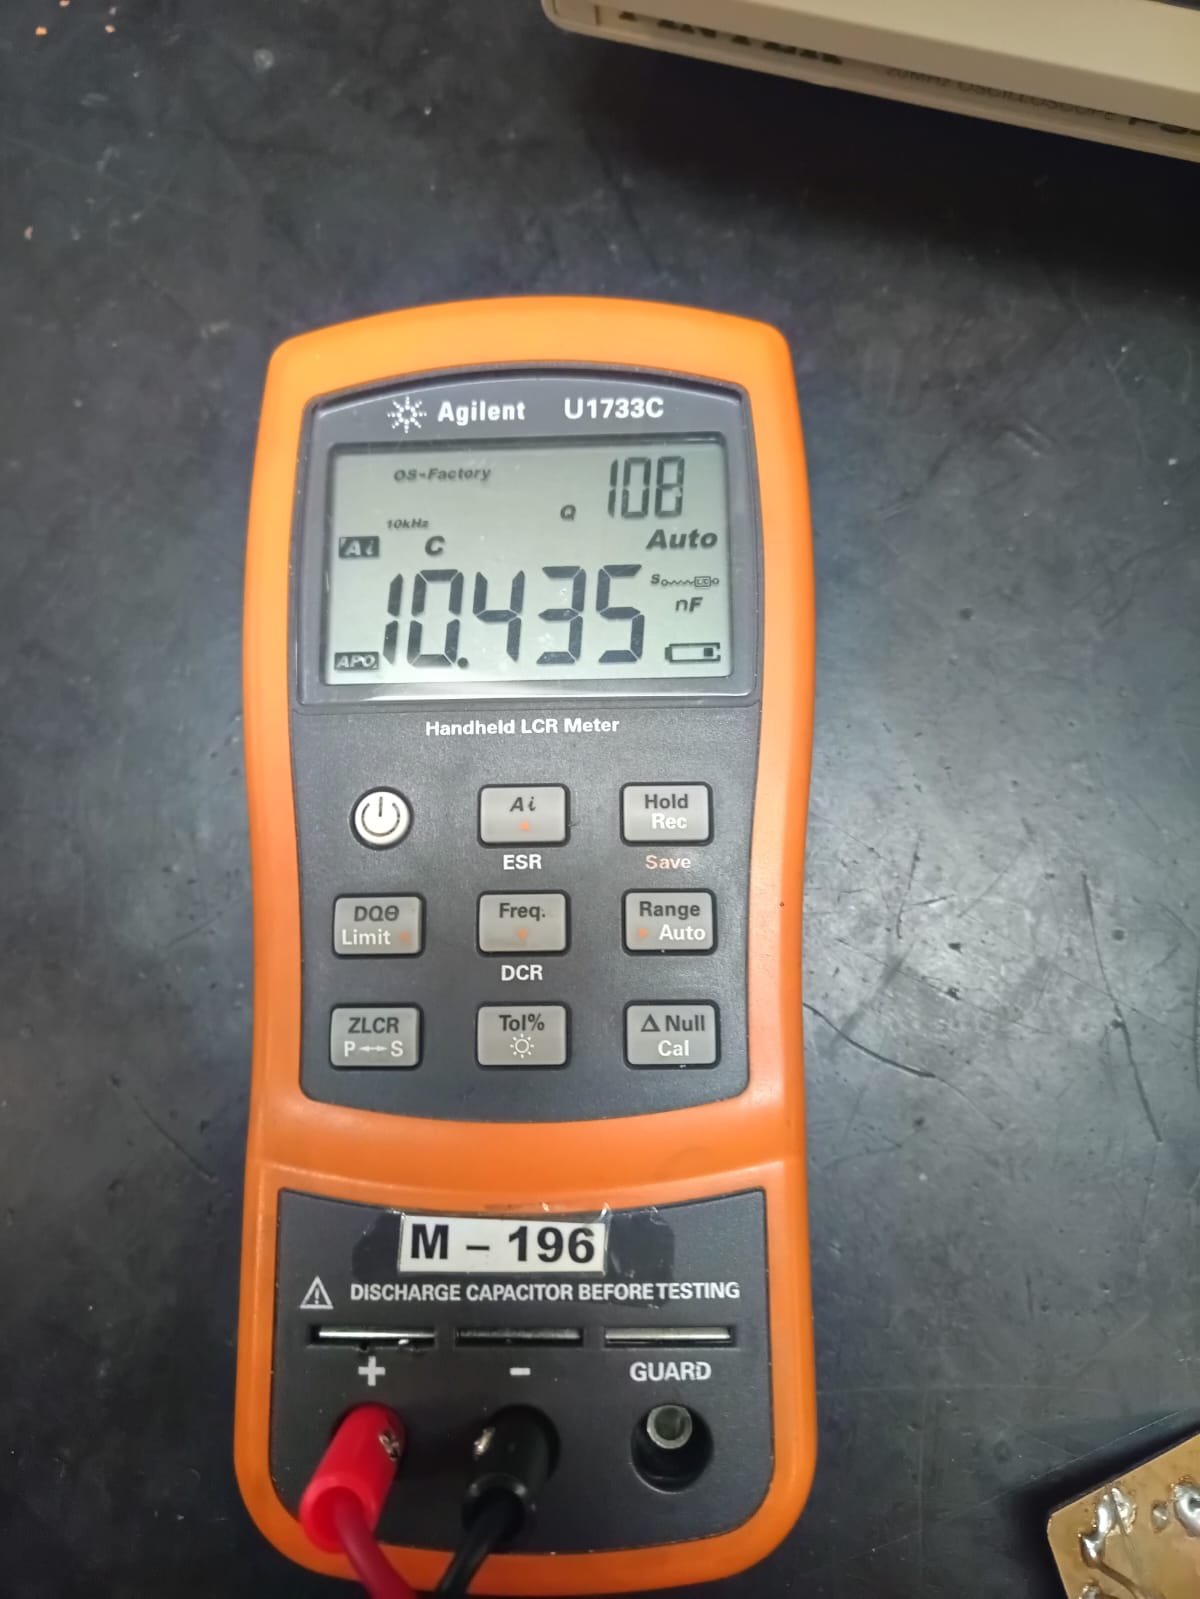
\includegraphics[width=\textwidth]{Imagenes/MedCapExp3.jpeg}
    \caption{Medición del capacitor}
    \end{minipage}
    \begin{minipage}{0.49\textwidth}
    \centering
    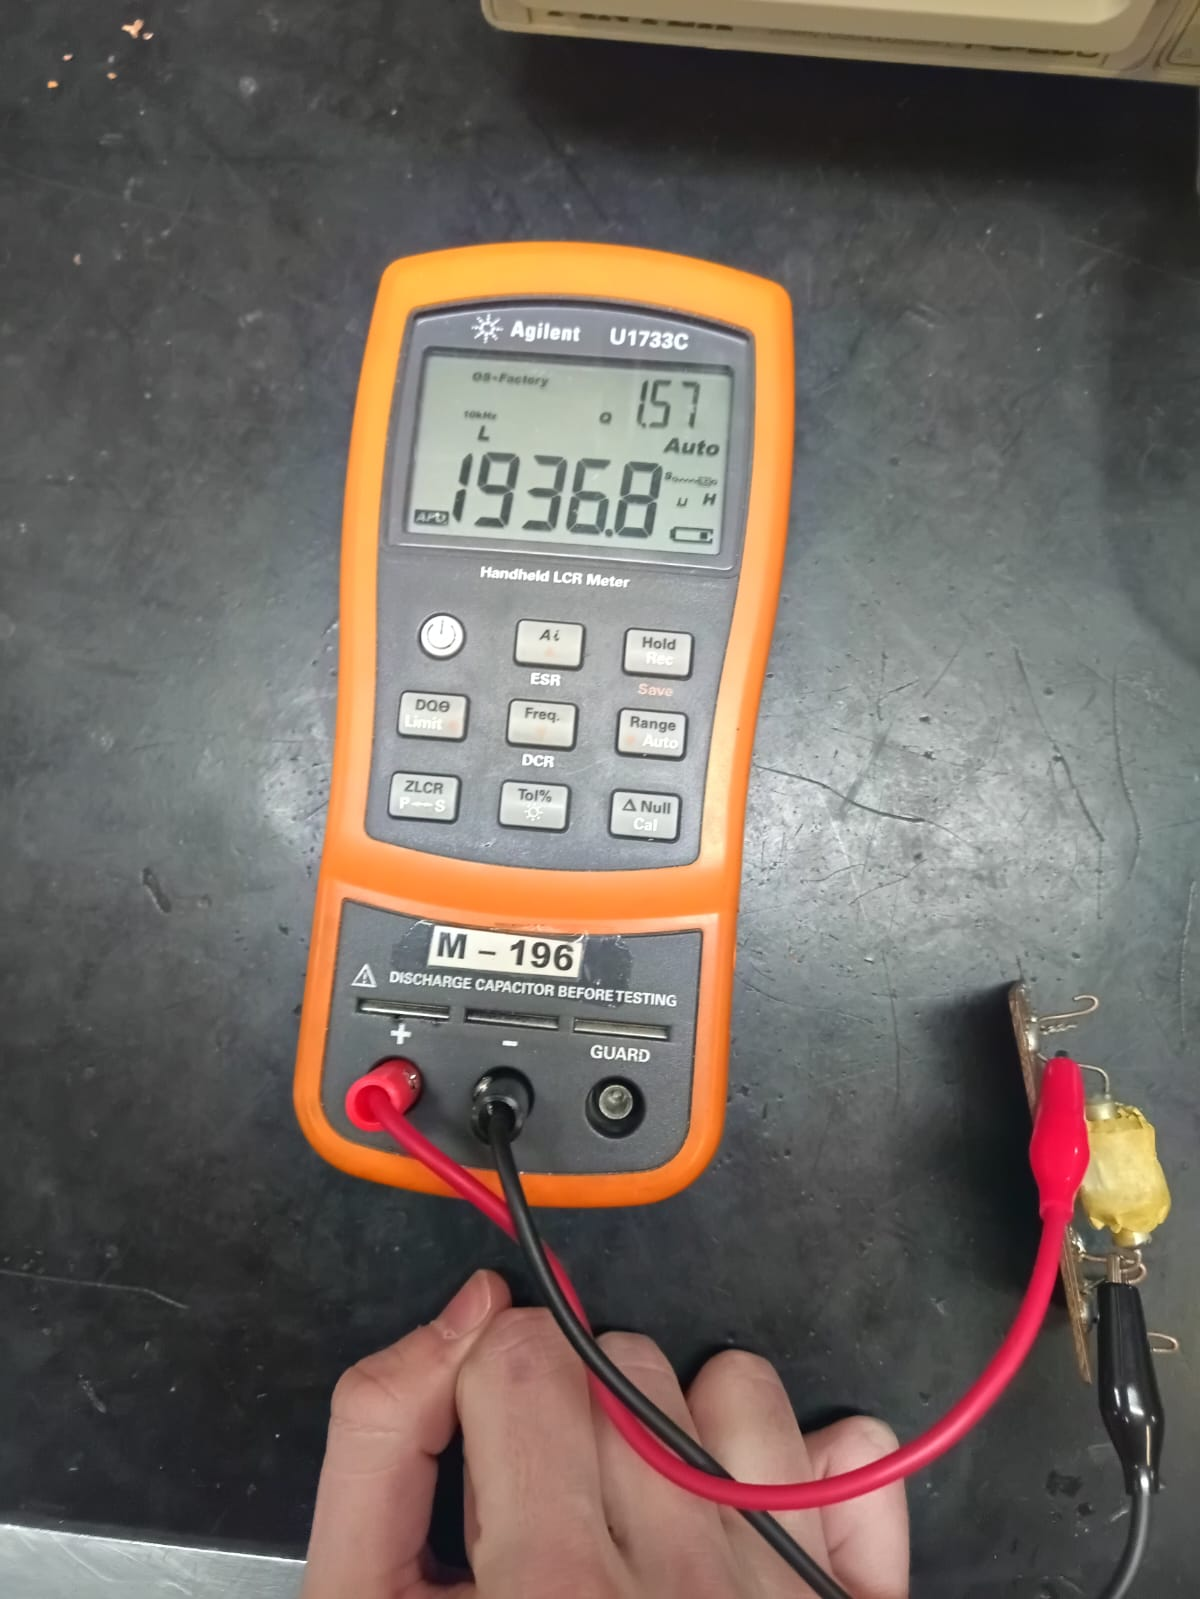
\includegraphics[width=\textwidth]{Imagenes/MedIndExp3.jpeg}
    \caption{Medición del inductor}
    \end{minipage}
\end{figure}